\item I recover the directory of staff in Tokyo-Fu by digitizing historical documents of the institution's directory of staff. The directory contains information on the position, title, occupation, and wage of all the staff in a given year.

\item I combine a deep neural network trained on historical Japanese documents and propriety OCR software to digitize the documents (Figure 2). After detecting the candidate of names using the OCR, I apply a Named Entity Recognition algorithm to find the objects with names.

\begin{figure}
    \centering
    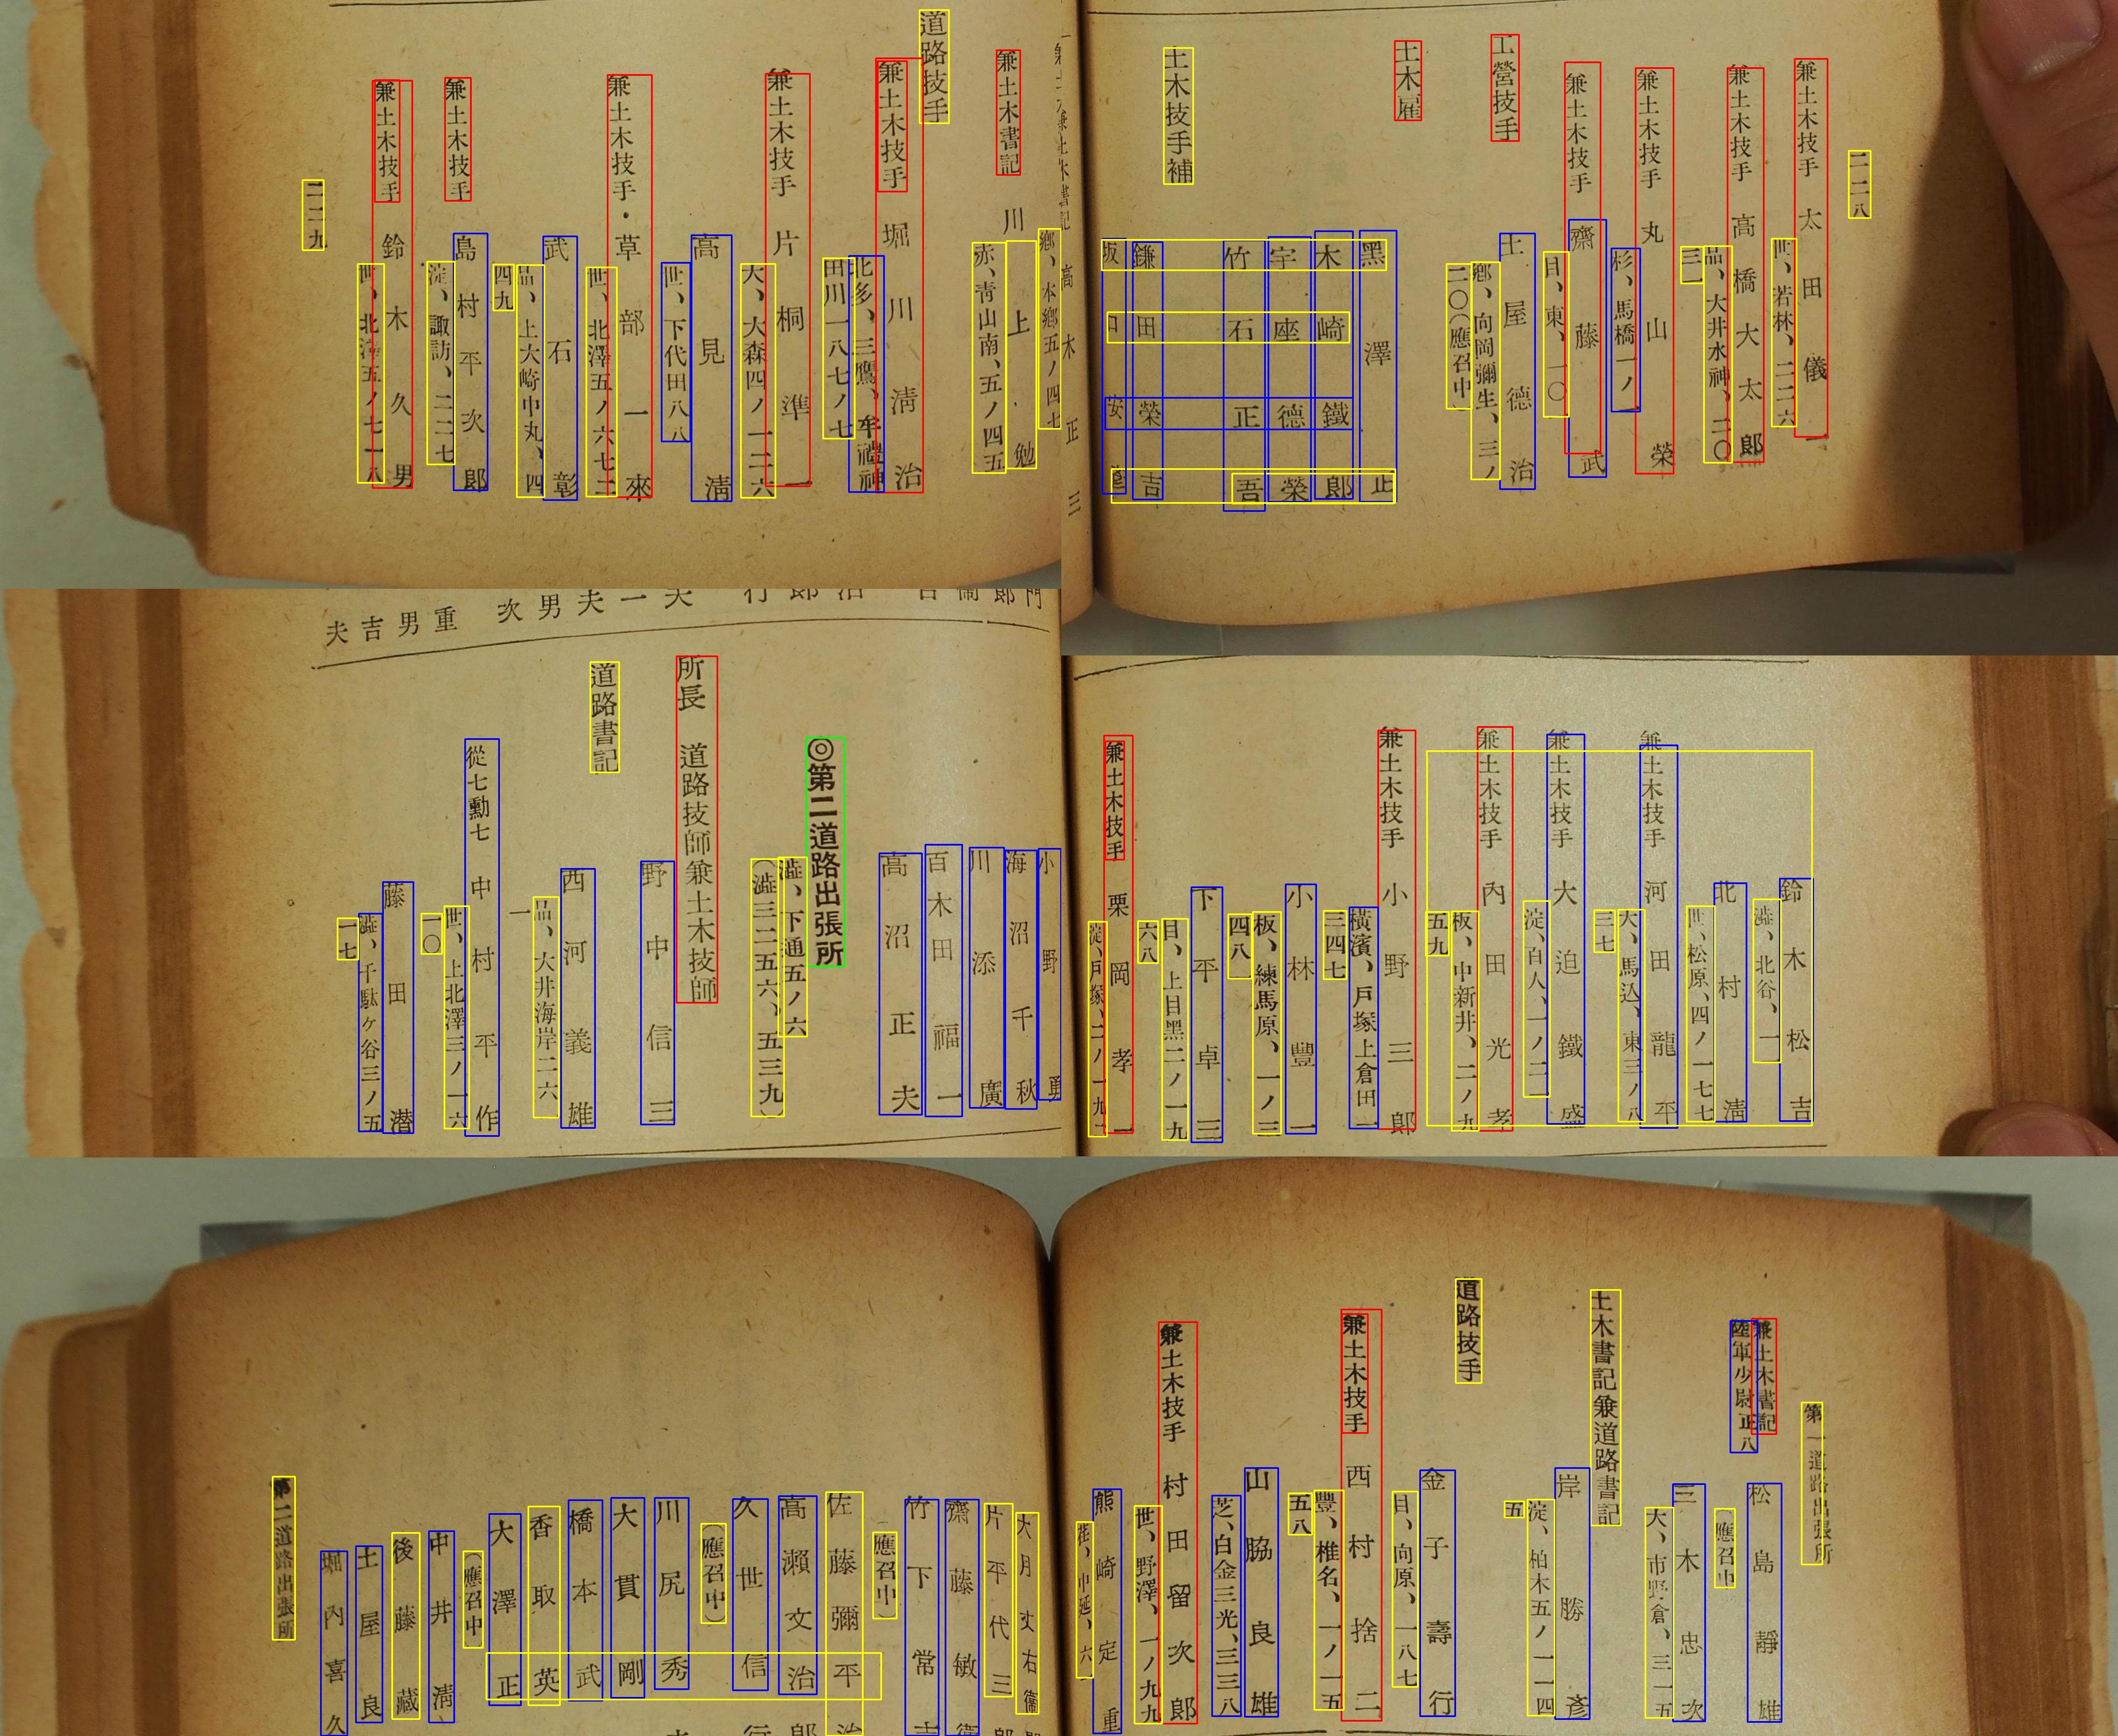
\includegraphics[width = \textwidth]{Data/Annotated_Page127.jpg}
    \caption{Example of OCR}
    \label{fig:enter-label}
\end{figure}